%%%%%%% DO NOT TOUCH IT! Or it might crash... dont come asking for support later ¯\_(ツ)_/¯. 
\documentclass[../../../main.tex]{subfiles}
\graphicspath{ {\subfix{../../../CTsettings/figures/}} {./figures/} {../figures/}}
%%%%%%% DO NOT TOUCH IT! Or it might crash... dont come asking for support later ¯\_(ツ)_/¯. 

\begin{document}
%%%%%%% DO NOT TOUCH IT! Or it might crash... dont come asking for support later ¯\_(ツ)_/¯. 
\onlyinsubfile{
    \renewcommand{\onlyinsubfile}[1]{}
    \renewcommand{\notinsubfile}[1]{#1}

    \renewcommand{\onlyonmainfile}[1]{}
    \renewcommand{\onlyonpartfile}[1]{}
    \renewcommand{\onlyonchapterfile}[1]{#1}
    \renewcommand{\onlyonsectionfile}[1]{}

    \gdef\CTMcalibrefontpath{../../../CTsettings/calibrefontfiles/}
    \setcalibrefont{\CTMcalibrefontpath}
    
    \fancypagestyle{plain}{\pagestyle{CTstylewithpage}}
    \pagestyle{CTstylewithpage}

}
%%%%%%% DO NOT TOUCH IT! Or it might crash... dont come asking for support later ¯\_(ツ)_/¯. 

\onlyonchapterfile{
}




\chapter{Potatoes are nice}


Gollum : What's taters, precious? What's taters, eh?

Sam : *Po-tay-toes!* Boil 'em, mash 'em, stick 'em in a stew... Lovely big golden chips with a nice piece of fried fish.

\lipsum[3-12]


\subfile{./potato_folder/section_monalisa}


\section{Local Section}

This is just for potato.

\begin{figure}[!htbp]
    \centering
    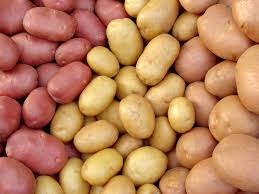
\includegraphics[width=0.5\textwidth]{./figures/potato_all.jpeg}
    \caption{Potato ALL}
    \label{fig:potato_all}
\end{figure}





\section{Table Section Example}

\begin{table}[!htbp]
    \centering
    \caption{Sample Table}
    \begin{tabular}{|c|c|c|}
        \hline
        \rowcolor[HTML]{C0C0C0} 
        \textbf{Column 1} & \textbf{Column 2} & \textbf{Column 3} \\ \hline
        Row 1, Cell 1     & Row 1, Cell 2     & Row 1, Cell 3     \\ \hline
        Row 2, Cell 1     & Row 2, Cell 2     & Row 2, Cell 3     \\ \hline
        Row 3, Cell 1     & Row 3, Cell 2     & Row 3, Cell 3     \\ \hline
    \end{tabular}
\end{table}

\begin{sidewaystable}[!htbp]
    \centering
    \caption{Sample Rotated Table}
    \begin{tabular}{|c|c|c|c|c|c|c|c|}
        \hline
        \rowcolor[HTML]{C0C0C0} 
        \textbf{Column 1} & \textbf{Column 2} & \textbf{Column 3} & \textbf{Column 4}  & \textbf{Column 5}  & \textbf{Column 6} & \textbf{Column 7}  & \textbf{Column 8} \\ \hline
        Row 1, Cell 1  & Row 1, Cell 2  & Row 1, Cell 3  & Row 1, Cell 4 & Row 1, Cell 5 & Row 1, Cell 6 & Row 1, Cell 7 & Row 1, Cell 8   \\ \hline
        Row 2, Cell 1  & Row 2, Cell 2  & Row 2, Cell 3  & Row 2, Cell 4 & Row 2, Cell 5 & Row 2, Cell 6 & Row 2, Cell 7 & Row 2, Cell 8   \\ \hline
        Row 3, Cell 1  & Row 3, Cell 2  & Row 3, Cell 3  & Row 3, Cell 4 & Row 3, Cell 5 & Row 3, Cell 6 & Row 3, Cell 7 & Row 3, Cell 8  \\ \hline
        Row 4, Cell 1  & Row 4, Cell 2  & Row 4, Cell 3  & Row 4, Cell 4 & Row 4, Cell 5 & Row 4, Cell 6 & Row 4, Cell 7 & Row 4, Cell 8   \\ \hline
        % ... add more rows as needed
    \end{tabular}
\end{sidewaystable}




\begin{table}[ht]
    \centering
    \caption{Non Rotated Table - that breakes page}
    \begin{tabular}{|c|c|c|c|c|c|c|c|}
        \hline
        \rowcolor[HTML]{C0C0C0} 
        \textbf{Column 1} & \textbf{Column 2} & \textbf{Column 3} & \textbf{Column 4}  & \textbf{Column 5}  & \textbf{Column 6} & \textbf{Column 7}  & \textbf{Column 8} \\ \hline
        Row 1, Cell 1  & Row 1, Cell 2  & Row 1, Cell 3  & Row 1, Cell 4 & Row 1, Cell 5 & Row 1, Cell 6 & Row 1, Cell 7 & Row 1, Cell 8   \\ \hline
        Row 2, Cell 1  & Row 2, Cell 2  & Row 2, Cell 3  & Row 2, Cell 4 & Row 2, Cell 5 & Row 2, Cell 6 & Row 2, Cell 7 & Row 2, Cell 8   \\ \hline
        Row 3, Cell 1  & Row 3, Cell 2  & Row 3, Cell 3  & Row 3, Cell 4 & Row 3, Cell 5 & Row 3, Cell 6 & Row 3, Cell 7 & Row 3, Cell 8  \\ \hline
        Row 4, Cell 1  & Row 4, Cell 2  & Row 4, Cell 3  & Row 4, Cell 4 & Row 4, Cell 5 & Row 4, Cell 6 & Row 4, Cell 7 & Row 4, Cell 8   \\ \hline
        % ... add more rows as needed
    \end{tabular}
\end{table}






\FloatBarrier % Prevent unresolved floats from floating beyond this point
\subfile{./potato_folder/section_algo.tex}



%%%%%%% DO NOT TOUCH IT! Or it might crash... dont come asking for support later ¯\_(ツ)_/¯. 
\onlyonchapterfile{
    \newpage
    \section{Bibliografia}
    \bibliographystyle{seg}
    \bibliography{references.bib}
}
%%%%%%% DO NOT TOUCH IT! Or it might crash... dont come asking for support later ¯\_(ツ)_/¯. 



\end{document}